\section{Aufbau der Visual Studio Solution}\label{aufbau}
Die Visual Studio Projektmappe f�r das \DevEnv\ besteht aus mehreren Projekten, die in mehreren Kategorien gruppiert sind. Abbildung~\ref{fig:solution} zeigt einen Screenshot des \emph{Solution Explorers} von Visual Studio und gibt einen �berblick �ber die verschiedenen Projekte.

Die Verzeichnis-Struktur des Projekts im Dateisystem entspricht nicht dem Visual Studio-Standard. Unterhalb des Hauptverzeichnisses gibt es drei weitere Verzeichnisse: bin, in dem alle kompilierten DLLs, die \emph{Executable} des Clients und das Knight-Sample liegen; Dependencies, in dem alle ben�tigten Bibliotheken liegen; und src, in dem der komplette Source Code liegt.

\begin{figure}[ht]
\centering
%trim=l b r t  	This option will crop the imported image by l from the left, b from the bottom, r from the right, and t  from the top. Where l, b, r and t are lengths. 
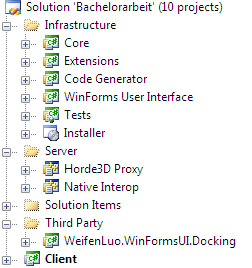
\includegraphics[scale=0.6]{images/Solution.png}
\caption{Aufbau der Visual Studio 2008 \emph{Solution}}\label{fig:solution}
\end{figure}

\subsubsection{Infrastructure}
In der Infrastruktur-Kategorie befinden sich die Projekte, die vom Client und vom Server gemeinsam benutzt werden, sowie der Code Generator und der \emph{Installer}. Alle Projekte dieser Kategorie sind in \Csharp\ geschrieben.

\begin{itemize}
	\item \textbf{Core} (DLL): Diese DLL enth�lt die Kern-Klassen des Systems. Dort befinden sich die Klassen und Interface-Definitionen f�r die Client-Server-Kommunikation, die \Horde-Klassen, die Klassen f�r das Profiling und die \Horde-Meldungen sowie \texttt{Horde3DCall} und \texttt{Horde3DDebugger}.
	
	\item \textbf{Extensions} (DLL): Dieses Projekt stellt einige n�tzliche Erweiterungen f�r das .NET Framework bereit, die vom \DevEnv\ an vielen Stellen verwendet werden.
	
	\item \textbf{Code Generator} (\emph{Executable}): Der Code Generator ist eine eigenst�ndige Anwendung zur Generierung der \Horde-\emph{Proxy}-Funktionen und -Klassen. Zur Laufzeit des Systems wird dieses Projekt nicht ben�tigt.
	
	\item \textbf{WinForms User Interface} (DLL): Diese \emph{Assembly} enth�lt die Implementierung des GUI-Frameworks unter Verwendung der Windows Forms-Klassen.
	
	\item \textbf{Tests} (DLL): Diese Bibliothek enth�lt \emph{Unit Tests} f�r das System. Derzeit gibt es allerdings nur Tests f�r das Parsen der XML-Dateien von Shader-Ressourcen.
	
	\item \textbf{Installer} (\emph{Executable}): Das Projekt erzeugt eine .msi-Datei f�r den Windows \emph{Installer}. Der \emph{Installer} kann das \DevEnv\ auf einem Computer installieren, aktualisieren und wieder l�schen. Alle Voraussetzungen -- .NET 3.5 SP1 und die Visual C++ \emph{Redistributable} f�r 32 Bit Systeme -- werden automatisch installiert.
\end{itemize}

\subsubsection{Server}
Die Server-Projekte sind .NET-\emph{Assemblies}, die in \C++/CLI geschrieben wurden. In \C++/CLI ist der Zugriff auf native Funktionen sowie die Verwendung von Zeigern einfacher und performanter als unter \Csharp. M�chte man diese \emph{Assemblies} debuggen, so ben�tigt man zun�chst eine \Horde-Anwendung, die vom \DevEnv\ gestartet wurde. Anschlie�end kann man die "`\emph{Attach Debugger}"'-Funktionalit�t von Visual Studio verwenden, um den Prozess der Anwendung zu debuggen. Zu beachten ist, dass die DLLs sowohl \emph{managed} als auch nativen Code enthalten. Der Debugger muss daher unbedingt auf "`\emph{mixed mode}"' gesetzt werden, da er ansonsten nur den nativen oder nur den \emph{managed} Teil des Codes sieht.

\begin{itemize}
	\item \textbf{Horde3D Proxy} (DLL): In dieser DLL befinden sich die \Horde-\emph{Proxy}-Funktionen sowie die globale Instanz der \texttt{Horde3DProxyHandler}-Klasse.
	
	\item \textbf{Native Interop} (DLL): Der Server f�hrt einige Aktionen durch, die sehr stark von der Win32-API abh�ngen und daher in \C++/CLI einfacher implementierbar sind. In dieser DLL befindet sich der komplette Code des \emph{Strategy Patterns} zum Anhalten der Anwendung und auch der Code zum Auslesen und Konvertieren des Inhalts eines \emph{Render Targets}.
\end{itemize}

\subsubsection{Third Party}
Zur Zeit befindet sich blo� das Projekt der Weifen Luo Winforms Docking Bibliothek in dieser Kategorie. Das \DevEnv\ verwendet zwar noch weitere Open Source Bibliotheken, diese wurden aber nicht modifiziert. In der \emph{Docking}-Bibliothek wurden hingegen ein paar kleine �nderungen vorgenommen, um das Aussehen der Shell an das von Visual Studio anzugleichen.

\subsubsection{Client}
Der Client ist das eigentliche ausf�hrbare Projekt des \DevEnvs. Vor der Kompilierung des Projekts werden die DLLs, die beim Starten des Servers in das Anwendungsverzeichnis kopiert werden m�ssen, in das \emph{Resources}-Verzeichnis des Client-Projekts kopiert. Der Compiler kompiliert dann die DLLs in die .exe-Datei als .NET-Ressource hinein. Soll der Server gestartet werden, so k�nnen die ben�tigten DLLs aus den Ressourcen ausgelesen werden. Damit entf�llt das fehleranf�llige Kopieren direkt aus dem Anwendungsverzeichnis der Shell.

Da die Verzeichnis-Struktur der \emph{Solution} nicht der Standardstruktur von Visual Studio entspricht, m�ssen zum Debuggen des Clients zwei Projekt-Einstellungen ge�ndert werden. In den Einstellungen muss im Abschnitt "`\emph{Debug}"' die "`\emph{Start Action}"' auf "`\emph{Start external program}"' gesetzt werden. Au�erdem muss der Pfad zur .exe-Datei im bin-Verzeichnis angegeben werden. Das "`\emph{Working Directory}"' muss ebenfalls auf das bin-Verzeichnis gesetzt werden.